% AAMAS 2013 Manuscript

% This file should be compiled with "aamas2013.cls" 
% ----------------------------------------------------------------------
% REMEMBER: After having produced the .bbl file,
% and prior to final submission, you *NEED* to 'insert'
% your .bbl file into your source .tex file so as to provide
% ONE 'self-contained' source file.
% ----------------------------------------------------------------------

%%%%%%%%%%%%%%%%%%%%%%%%%%%%%%%%%%%%%%%%%%%%%%%%%%%%%%%%%%%%%%%%%%%%%%%%%%%%%%
% STYLE NOTES
%
% TENSE AND VOICE
% * Actual experimental events
% 	We wrote descriptions of actual experimental events using past tense, in 
%	active voice, as the first person plural.
%
% * All other contexts
%	We write all other text using present tense, in active voices, as the
%	the first person plural.  
%
% CONVENTIONS
% flapping-wing, small-scale, lightweight, MAV
%
%%%%%%%%%%%%%%%%%%%%%%%%%%%%%%%%%%%%%%%%%%%%%%%%%%%%%%%%%%%%%%%%%%%%%%%%%%%%%%
% SETUP
\documentclass{aamas2013}

%----------------------------------------------------------------------------%
% PACKAGES
\usepackage{color}
\usepackage[pdftex]{hyperref}

%----------------------------------------------------------------------------%
% METADATA
\def \papertitle{Cooperative Control for Narrow Passage Traversal with an 
Ornithopter Micro Air Vehicle and Lightweight Ground Station}
\def \paperkeywords{AAMAS proceedings, multiagent systems, cooperative control, 
particle filter, micro air vehicle, ground station, visual servoing, pose 
estimation, flapping wing, ornithopter, biomimetic}
\def \paperterms{Algorithms, Performance, Design, Experimentation}
\def \paperauthors{Ryan C. Julian, Cameron J. Rose, Humphrey Hu, and Ronald S. Fearing}

% Set title
\title{\papertitle}

% PDF bookmarks
\definecolor{linkCol}{gray}{0.25}
\hypersetup{
    pdftitle={\papertitle},
    pdfauthor={\paperauthors},
    pdfsubject={\paperterms},
    pdfkeywords={\paperkeywords},
    pdfpagemode=UseOutlines, bookmarksopen, bookmarksnumbered,
    colorlinks, linkcolor=linkCol, citecolor=linkCol, urlcolor=linkCol
}

%----------------------------------------------------------------------------%
% pdfLatex clean-up 
\pdfpagewidth=8.5truein
\pdfpageheight=11truein

\begin{document}

%%%%%%%%%%%%%%%%%%%%%%%%%%%%%%%%%%%%%%%%%%%%%%%%%%%%%%%%%%%%%%%%%%%%%%%%%%%%%%
% AUTHORS

%% Paper number instead of authors
%\numberofauthors{1}
%\alignauthor Paper  XXX

\numberofauthors{4}
\author{
\alignauthor Ryan C. Julian\\
       \affaddr{Department of EECS}\\
       \affaddr{Univ. of California, Berkeley}\\
       \affaddr{Berkeley, CA 94720}\\
       \email{ryanjulian@berkeley.edu}
\alignauthor Cameron J. Rose\\
       \affaddr{Department of EECS}\\
       \affaddr{Univ. of California, Berkeley}\\
       \affaddr{Berkeley, CA 94720}\\
       \email{c\_rose@eecs.berkeley.edu}
\alignauthor Humphrey Hu\\
       \affaddr{Robotics Institute}\\
       \affaddr{Carnegie Mellon University}\\
       \affaddr{Pittsburgh, PA 15213}\\
       \email{humhu@cmu.edu}
\and
\alignauthor Ronald S. Fearing\\
       \affaddr{Department of EECS}\\
       \affaddr{Univ. of California, Berkeley}\\
       \affaddr{Berkeley, CA 94720}\\
       \email{ronf@eecs.berkeley.edu}
}

%%%%%%%%%%%%%%%%%%%%%%%%%%%%%%%%%%%%%%%%%%%%%%%%%%%%%%%%%%%%%%%%%%%%%%%%%%%%%%
% TITLE
\maketitle

%%%%%%%%%%%%%%%%%%%%%%%%%%%%%%%%%%%%%%%%%%%%%%%%%%%%%%%%%%%%%%%%%%%%%%%%%%%%%%
% ABSTRACT
\begin{abstract}
The power, size, and weight constraints of micro air vehicles (MAVs) limit 
their on-board sensing and computational resources. Ground vehicles have 
less mobility than MAVs, but relaxed size constraints and typically more 
computing power, creating opportunities for cooperation. In this work, we 
demonstrate cooperative target-seeking between a 13 gram ornithopter MAV 
and a lightweight ground station using computer vision.

We also introduce a new ornithopter MAV, the 13 gram H$^2$Bird. It 
features clap and fling wings, improves upon a previous design by 
utilizing a carbon fiber airframe, tail rotor, and elevator, and carries a 
payload of 2.8 grams. We augment the ornithopter's built-in 
gyroscope-based control with a ground station, which has power and weight 
requirements appropriate for deployment on 30 gram a ground vehicle. The ground 
station provides heading estimates to the ornithoper by running a 
real-time motion tracking algorithm on a live video stream. This allows 
the ornithopter to reliably negotiate flight through narrow openings.

We demonstrate the performance of the location estimation and navigation 
algorithms. We model the backwards-reachable region for successfully 
navigating through narrow openings. Finally, we verify this model through 
with collected in experiments with window traversal.
\end{abstract}
%%%%%%%%%%%%%%%%%%%%%%%%%%%%%%%%%%%%%%%%%%%%%%%%%%%%%%%%%%%%%%%%%%%%%%%%%%%%%%
% ACM METADATA

% Note that the category section should be completed after reference to 
% the ACM Computing Classification Scheme available at
% http://www.acm.org/about/class/1998/.
% A category including the fourth, optional field follows...
%\category{D.2.8}{Software Engineering}{Metrics}[complexity measures, 
% performance measures]
\category{I.2.9}{Robotics}{Autonomous Vehicles}
\category{I.2.9}{Robotics}{Distributed Artificial Intelligence}[Multiagent Systems]
\category{I.2.9}{Robotics}{Vision and Scene Understanding}[Motion]

% General terms should be selected from the following 16 terms: 
% Algorithms, Management, Measurement, Documentation, Performance, 
% Design, Economics, Reliability, Experimentation, Security, 
% Human Factors, Standardization, Languages, Theory, Legal Aspects, 
% Verification.
\terms{\paperterms}

% Keywords are your own choice of terms you would like the paper to be indexed 
% by.
\keywords{\paperkeywords}

%%%%%%%%%%%%%%%%%%%%%%%%%%%%%%%%%%%%%%%%%%%%%%%%%%%%%%%%%%%%%%%%%%%%%%%%%%%%%%
\section{Introduction}
%TODO(ryan)
The power, size, and weight constraints of micro air vehicle (MAV) 
platforms significantly limit on-board sensing and computational 
resources, and thus the complexity of the control and state estimation 
algorithms which can be executed on-board. These constraints are 
particularly severe for flapping wing MAVs offer the promise of superior 
safety, efficiency, and noise profile to rotor craft MAVs, but at the 
expense of payload weight.

\begin{figure}[!tb]
\centering
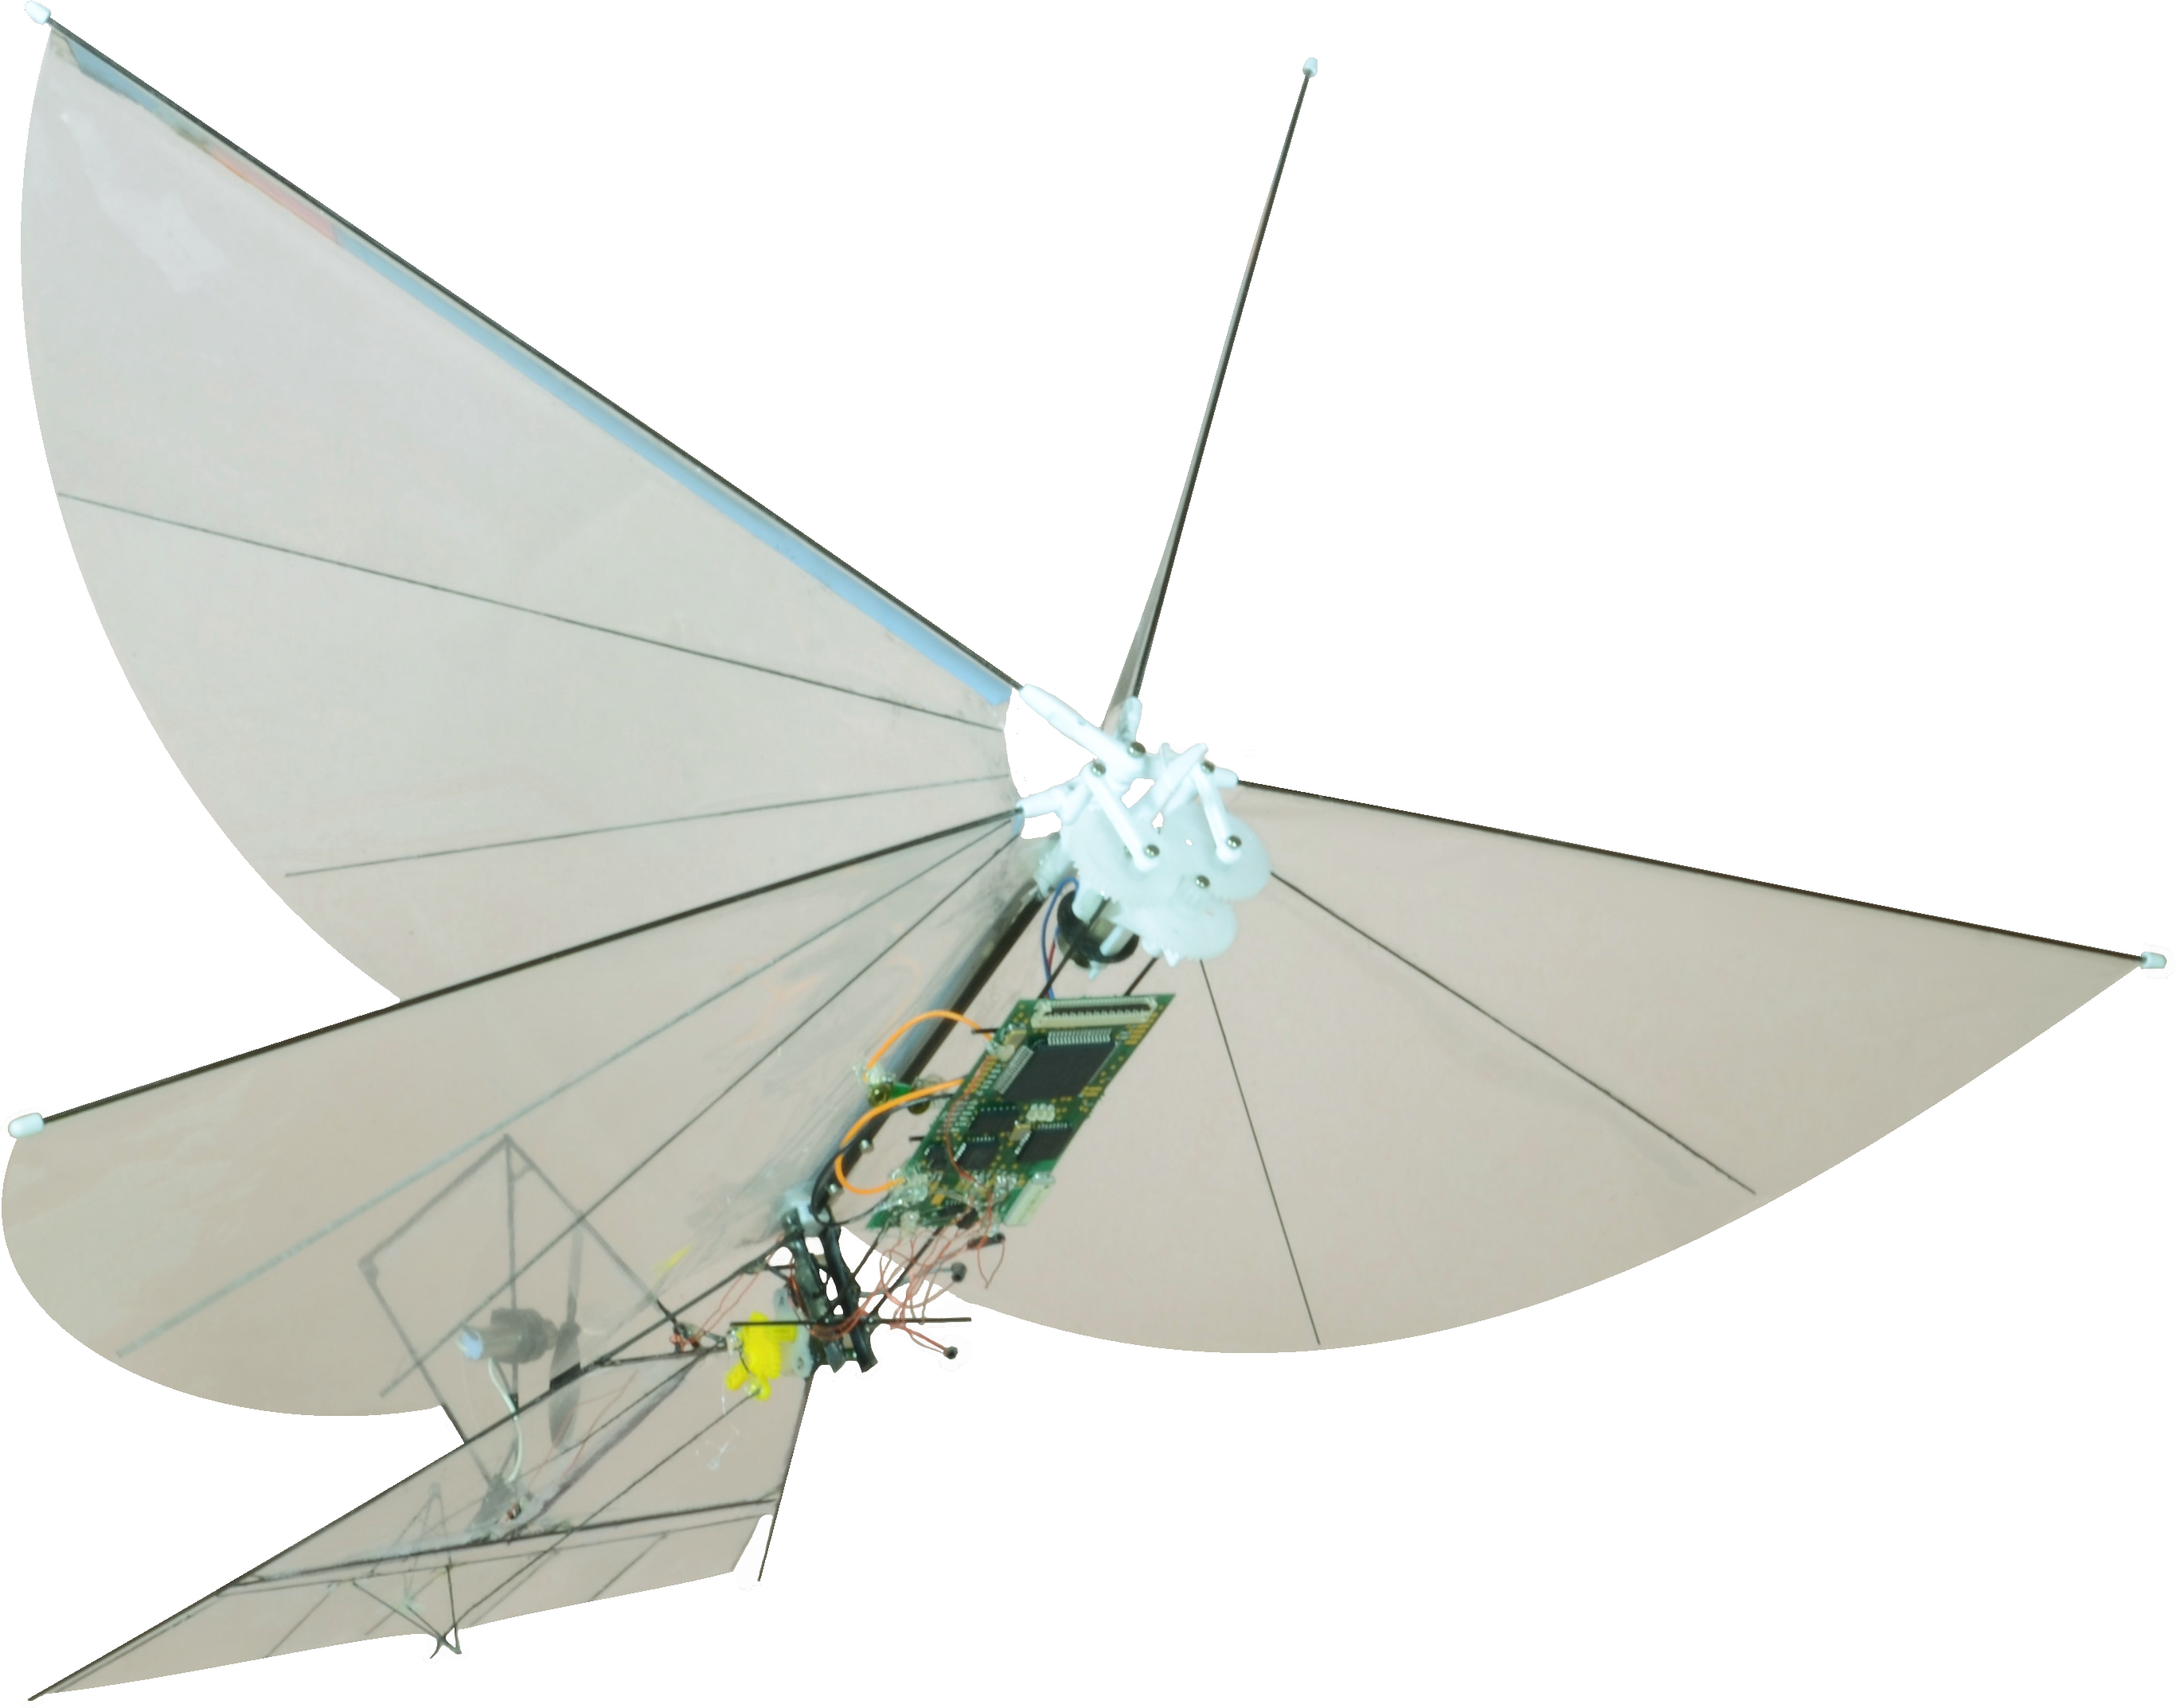
\includegraphics[width=\linewidth]{figures/h2bird.png}
\caption{H$^2$Bird Ornithopter MAV}
\label{fig:h2bird}
\end{figure}

%%%%%%%%%%%%%%%%%%%%%%%%%%%%%%%%%%%%%%%%%%%%%%%%%%%%%%%%%%%%%%%%%%%%%%%%%%%%%%
\section{Robotic and Vision Platforms}
%TODO ryan

%----------------------------------------------------------------------------%
\subsection{H$^2$Bird Ornithoper MAV}
%TODO(humphrey)
The flying platform used in this experiment is the H$^2$Bird flapping wing 
MAV. Built around the Silverlit I-Bird RC flyer power train and clap-fling 
wings, the H$^2$Bird has a wingspan of [40?] cm and has a flight weight of 
13 grams. A tail propeller and servo-controlled tail elevator provide 
control in the yaw and pitch axes. An on-board electronics package comprises 
a 40 MIPS microprocessor, 6 DOF IMU, IEEE 802.15.4 radio, VGA camera, and motor 
drivers with a 90 mAh lithium polymer battery for autonomous flight. In 
routine flight, the H$^2$Bird averages [insert speed] m/s ground speed and 
can operate for approximately 10 minutes.

%TODO footnote for Silverlit I-Bird
%TODO measure wingspan
%TODO ground speed

%----------------------------------------------------------------------------%
\subsection{Ground Station Computer Vision Platform}
%TODO ryan

%%%%%%%%%%%%%%%%%%%%%%%%%%%%%%%%%%%%%%%%%%%%%%%%%%%%%%%%%%%%%%%%%%%%%%%%%%%%%%

%%%%%%%%%%%%%%%%%%%%%%%%%%%%%%%%%%%%%%%%%%%%%%%%%%%%%%%%%%%%%%%%%%%%%%%%%%%%%%
\section{System Concept and Algorithms}
%TODO ryan

\begin{figure}[tb]
\centering
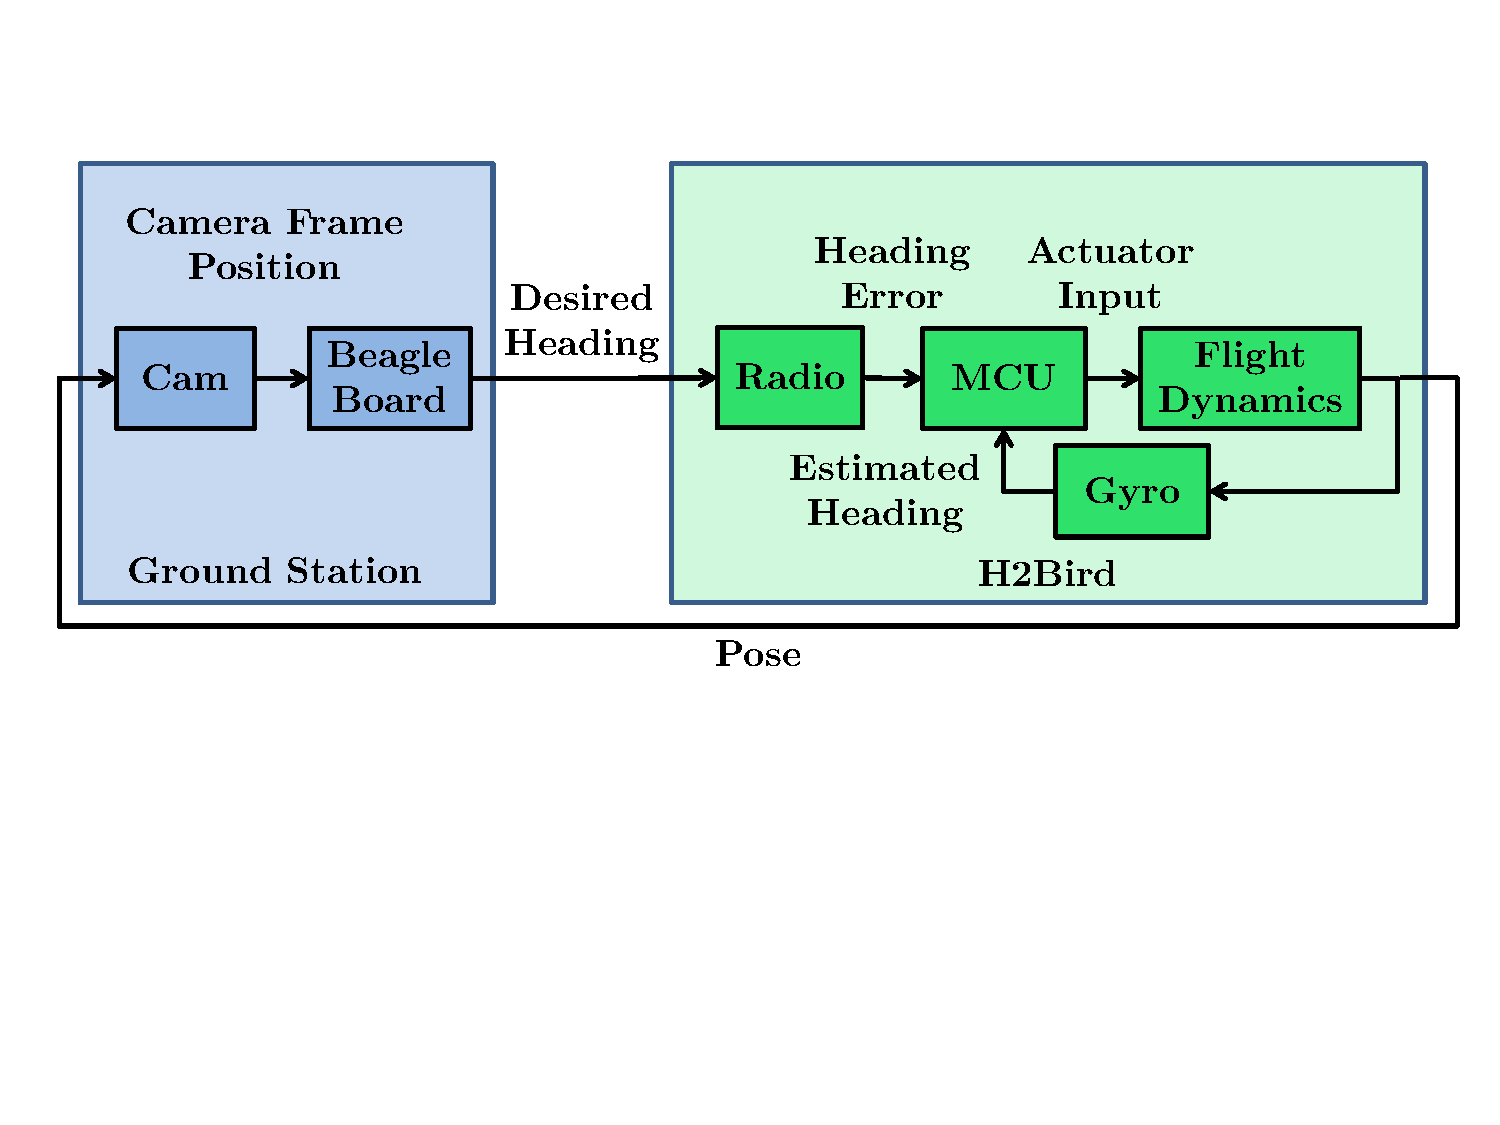
\includegraphics[width=\linewidth]{figures/process_flow.pdf}
\caption{Process flow diagram for the cooperative control system.}
\label{fig:process_flow}
\end{figure}

%----------------------------------------------------------------------------%
\subsection{Ornithoper Flight Control}

\begin{figure}[tb]
\centering
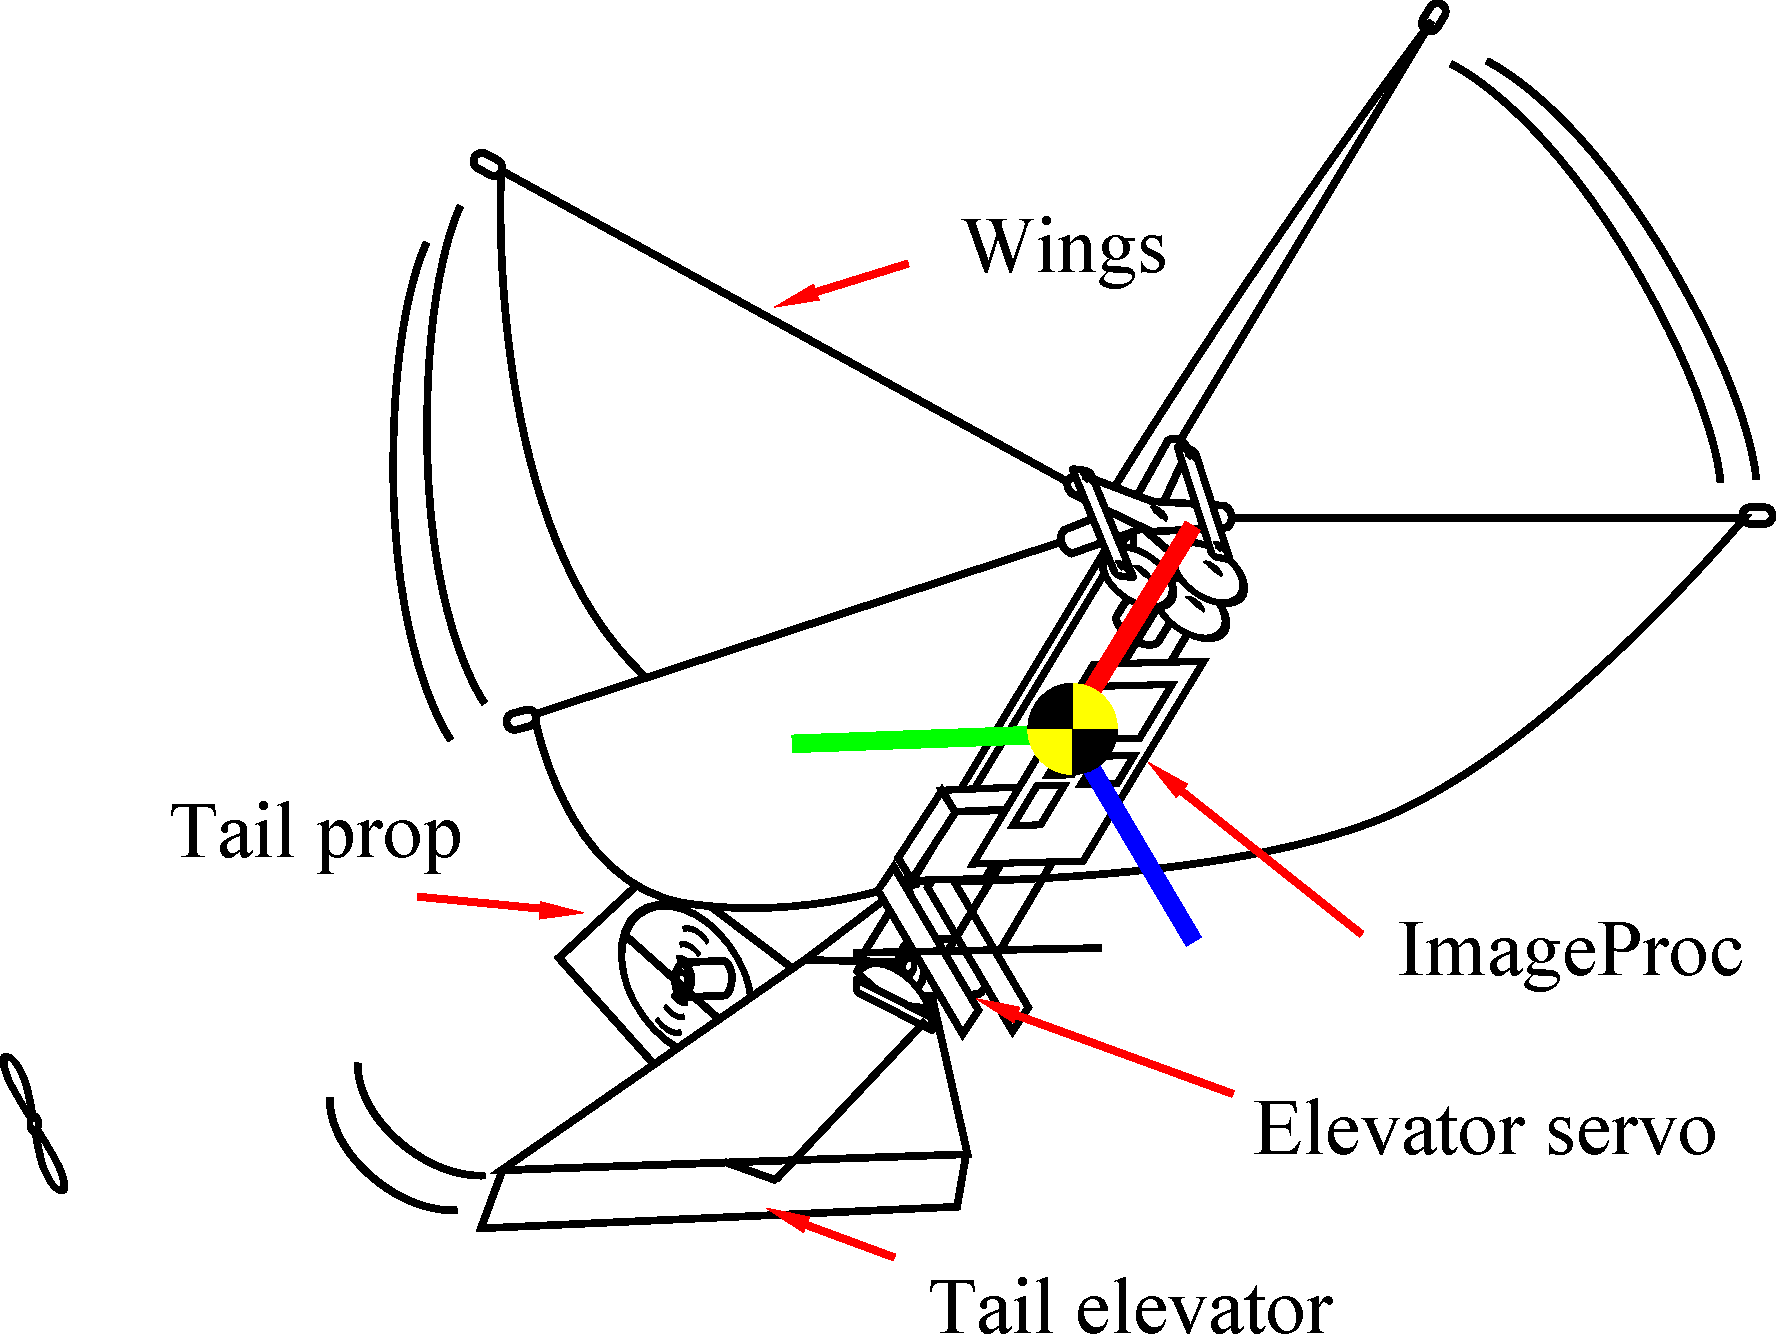
\includegraphics[height=150pt]{figures/h2bird_axes.pdf}
\caption{H$^2$Bird Ornithopter with flight control axes}
\label{fig:h2Bird_axes}
\end{figure}

Rudimentary attitude control for the H$^2$Bird runs on-board. It estimates 
pose by naively integrating the IMU and depending on PID for control. The 
simplistic nature of our state estimation and control is due to the 
stringent resource constraints applied by the platform.

We use simple controllers to actuate the H$^2$Bird's wing beat frequency, 
tail rotor, and tail elevator, which we designed to actuate thrust, yaw, 
and pitch respectively.

Due to the high pitch angles experienced by the H$^2$Bird, we use a 
quaternion representation of vehicle pose to avoid the numerical 
instabilities of Euler angle representations. This choice of pose 
representation also lends itself well to remote guidance, as relative body 
and world coordinate angular displacements can be represented compactly 
with quaternion multiplication.~\cite{bowman:reasoning} 

Given a reference pose $q$, we define the error $q_e$ as the rotation 
required to reach the reference pose from the measured pose. We then 
linearise the error quaternion to produce body axis angular errors as as 
inputs to the attitude controllers. 

Three independent proportional-integral-derivative controllers commanding 
the wing thrust, elevator, and tail propeller. We use this independent PID 
controller architecture for simplicity in tuning and implementation, and 
because it demonstrates acceptable performance in the absence of a system 
model.

\begin{equation}
\label{quat_error}
q_e = q'\otimes q_r
\end{equation}
\begin{equation}
\label{quat_angle}
\alpha = 2acos(q_{e,w})
\end{equation}
\begin{equation}
\label{quat_linearize}
Q_e = \alpha*q_e/sin(\alpha /2)
\end{equation}

%----------------------------------------------------------------------------%
\subsection{Pose Estimation}
%TODO ryan

%----------------------------------------------------------------------------%
\subsection{Visual Servoing}
%TODO ryan

%TODO trim PDF
\begin{figure}[tb]
\centering
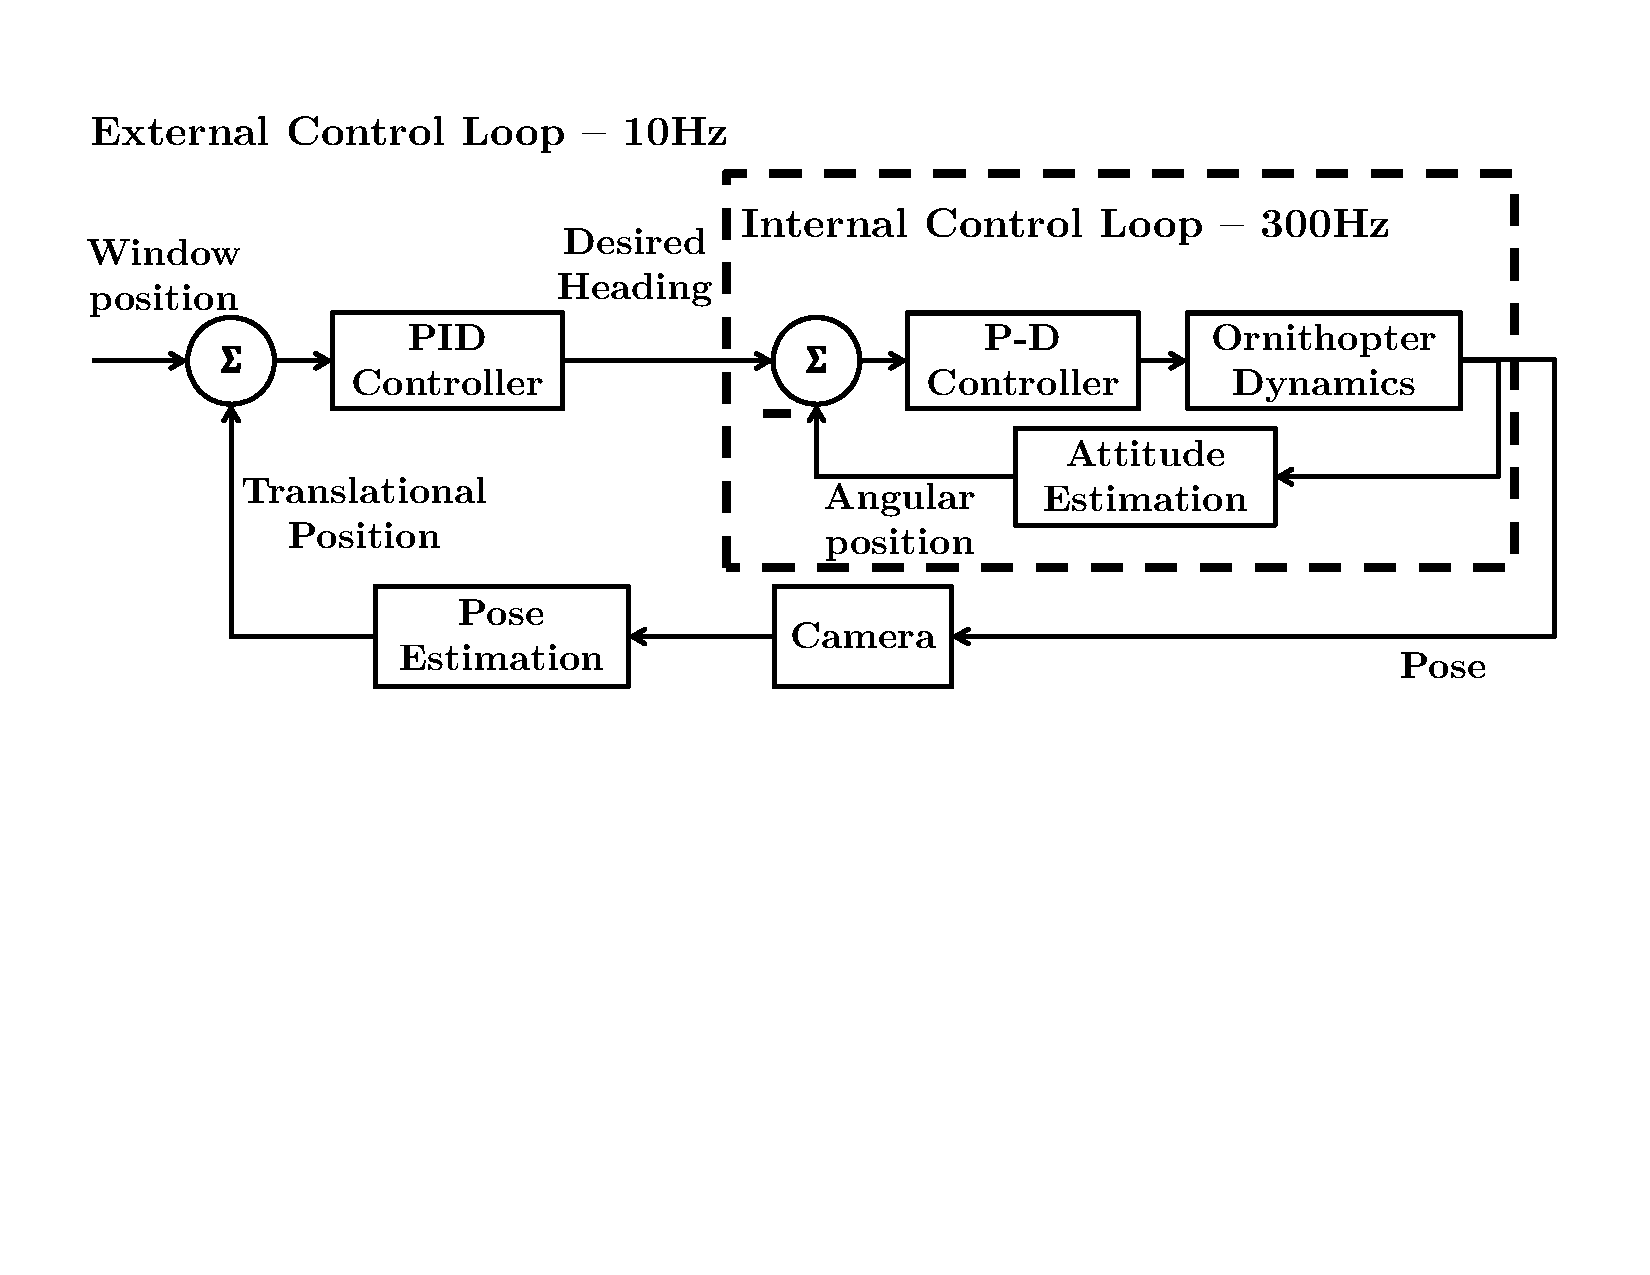
\includegraphics[width=\linewidth]{figures/block_diagrams.pdf}
\caption{Overall block diagram of cooperative control}
\label{fig:block_diagram}
\end{figure}

\begin{figure}[tb]
\centering
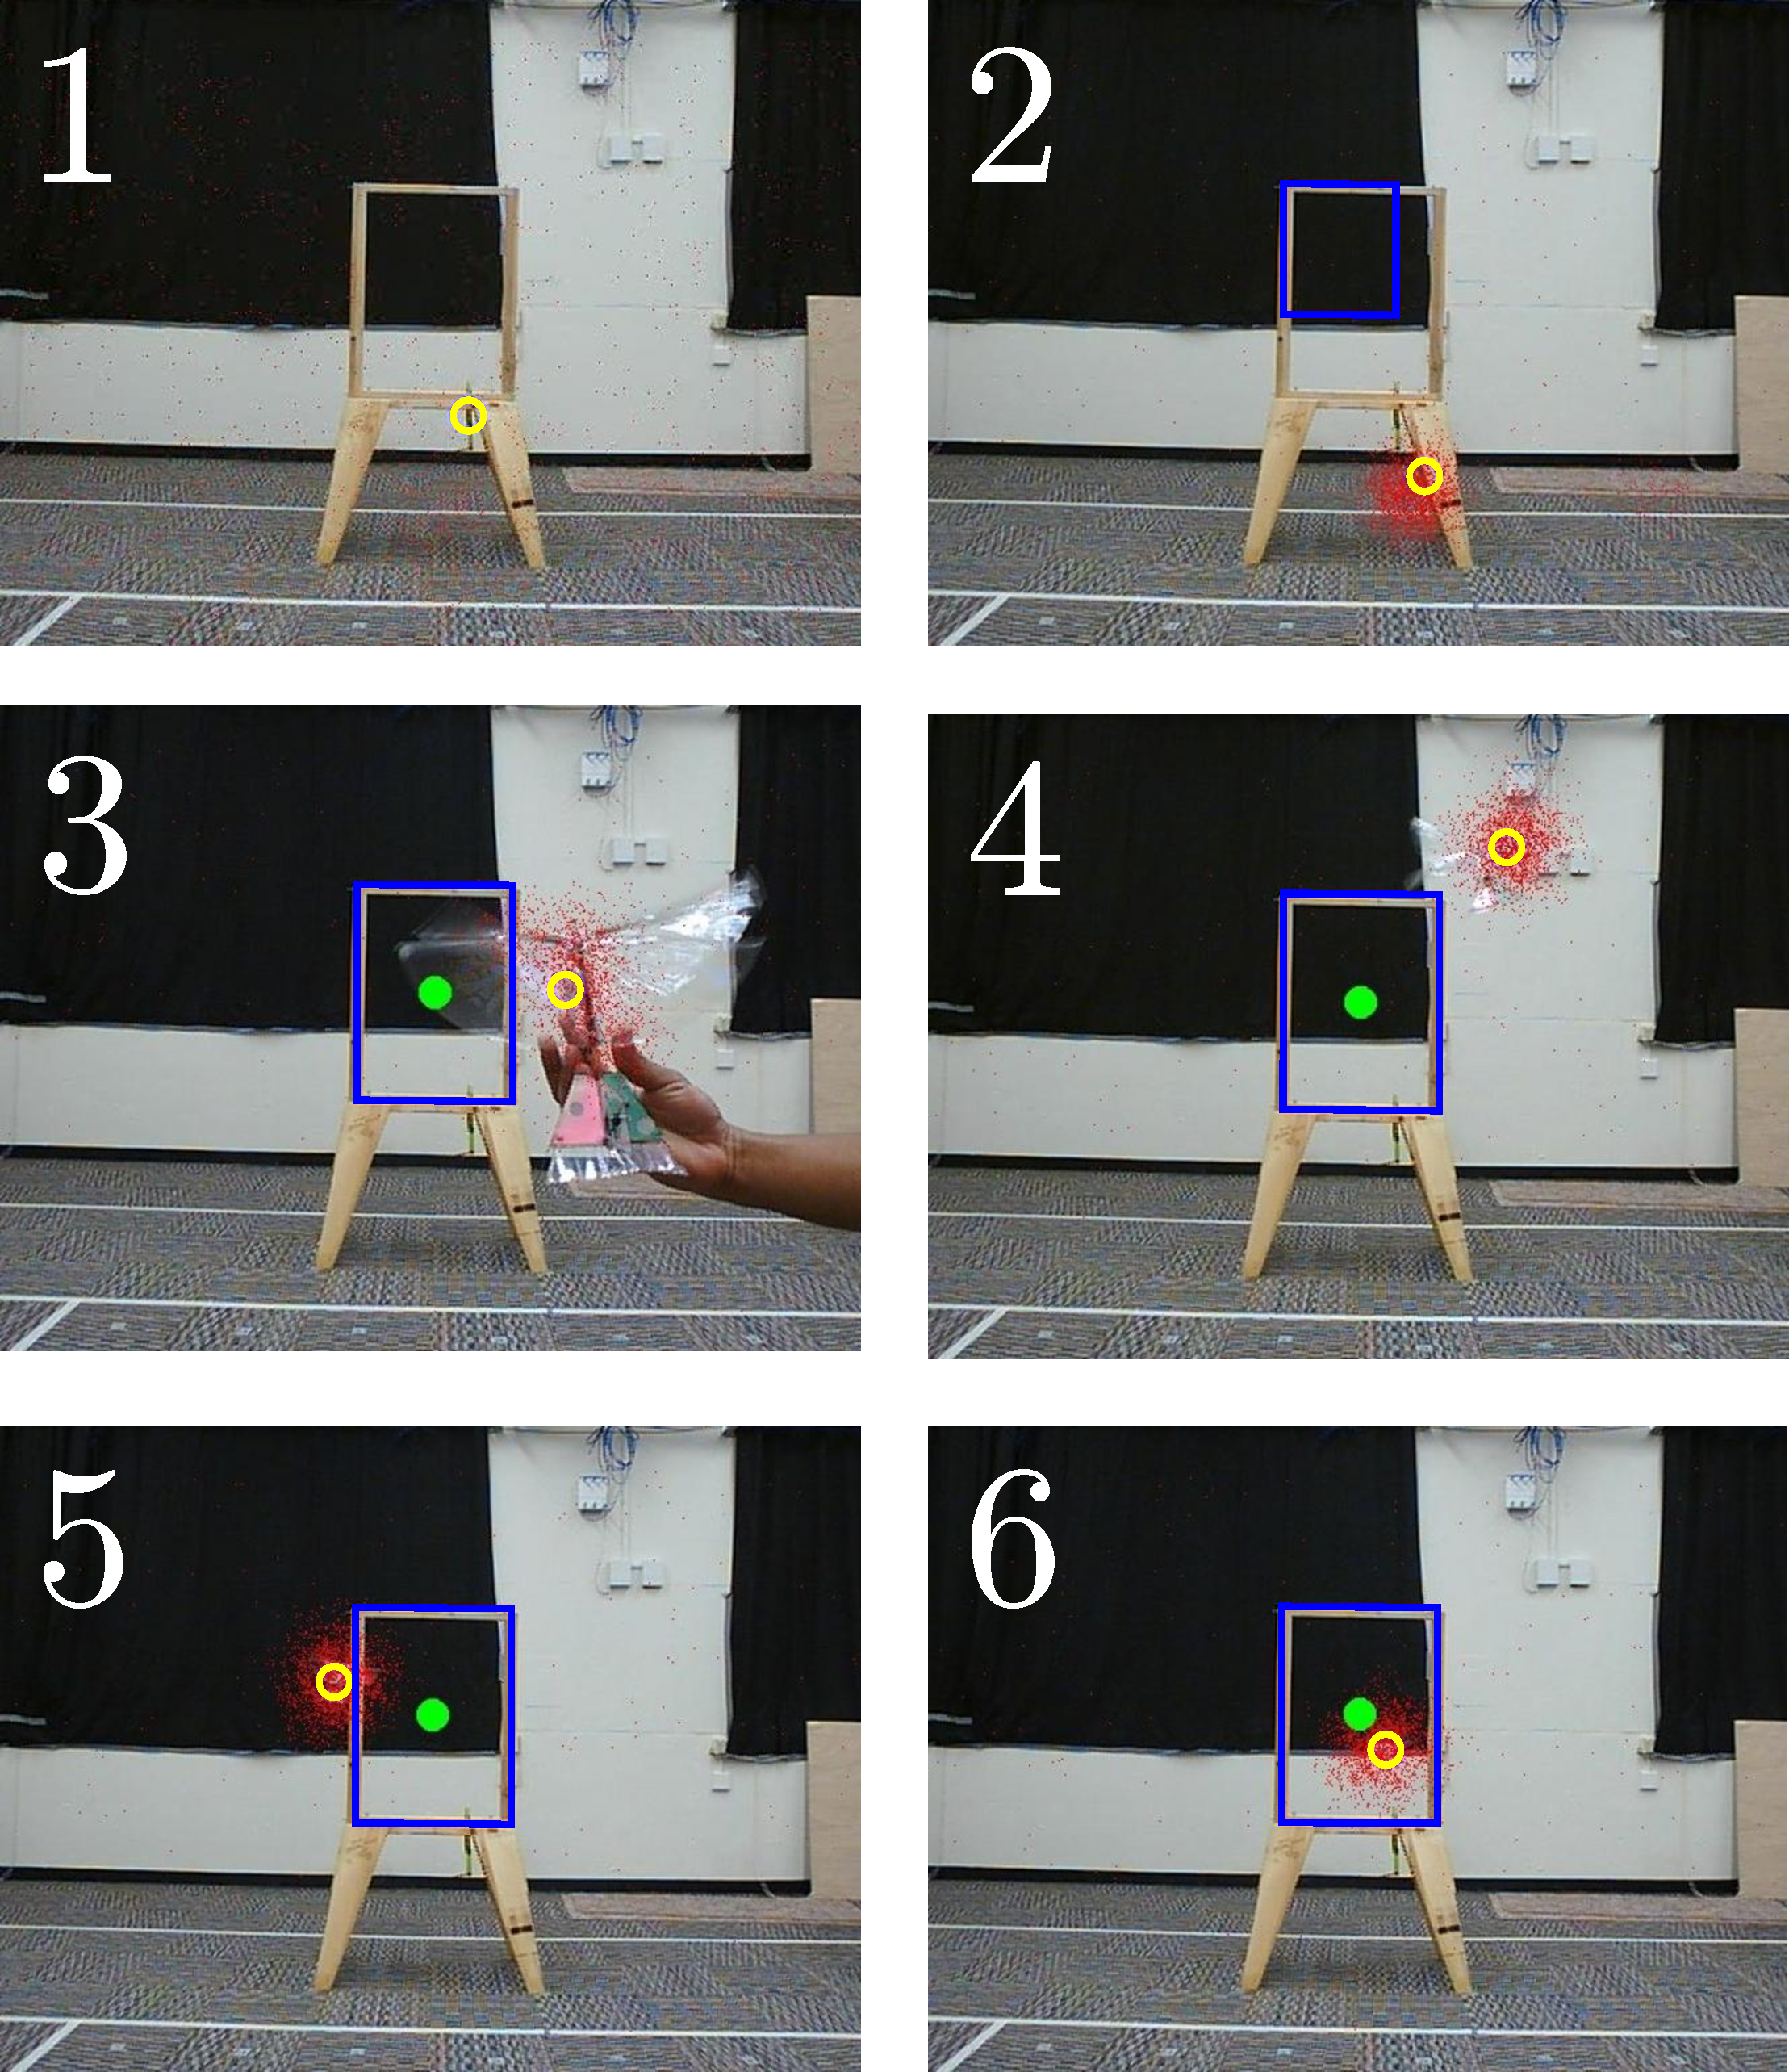
\includegraphics[width=\linewidth]{figures/pf_screencap.pdf}
\caption{Frame sequence from video feed used for tracking, showing 
particles and state estimate}
\label{fig:pf_screencap}
\end{figure}

%%%%%%%%%%%%%%%%%%%%%%%%%%%%%%%%%%%%%%%%%%%%%%%%%%%%%%%%%%%%%%%%%%%%%%%%%%%%%%

%%%%%%%%%%%%%%%%%%%%%%%%%%%%%%%%%%%%%%%%%%%%%%%%%%%%%%%%%%%%%%%%%%%%%%%%%%%%%%
\section{Experiments}
%TODO ryan

\begin{figure}[tb]
\centering
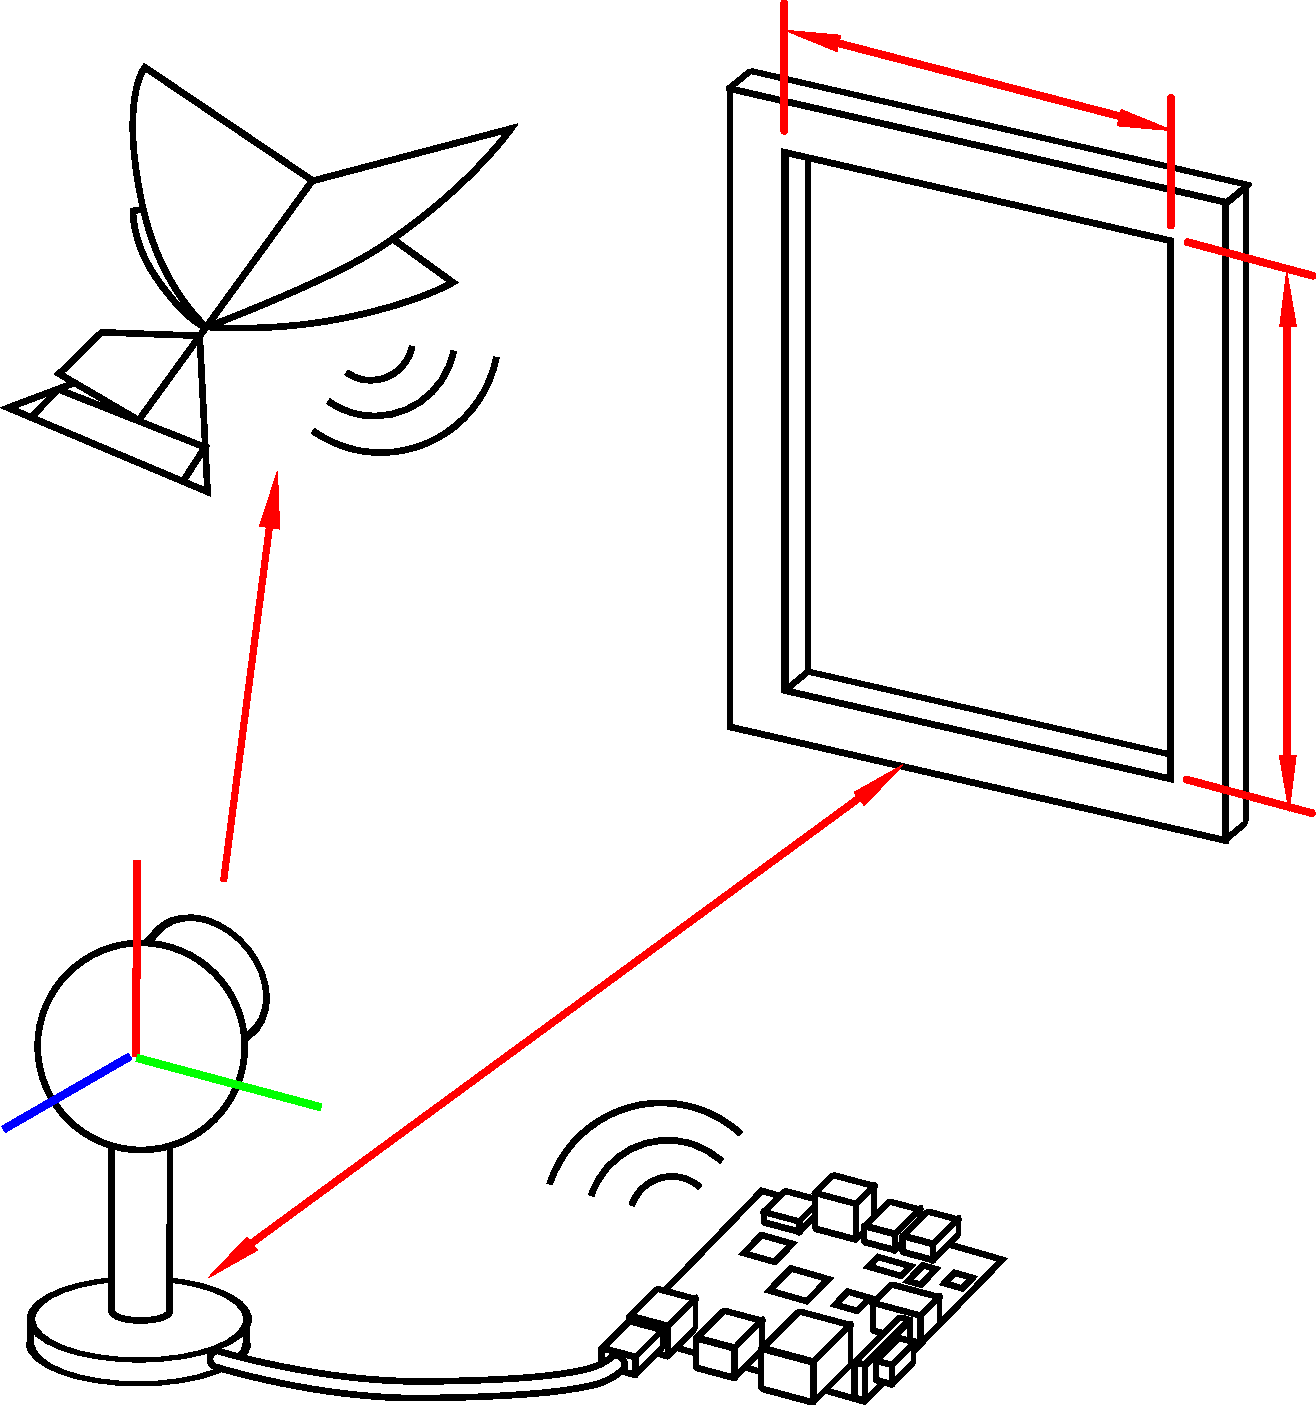
\includegraphics[width=\linewidth]{figures/experiment_cartoon.pdf}
\caption{Conceptual sketch of experimental environment.}
\label{fig:experiment_cartoon}
\end{figure}

%%%%%%%%%%%%%%%%%%%%%%%%%%%%%%%%%%%%%%%%%%%%%%%%%%%%%%%%%%%%%%%%%%%%%%%%%%%%%%

%%%%%%%%%%%%%%%%%%%%%%%%%%%%%%%%%%%%%%%%%%%%%%%%%%%%%%%%%%%%%%%%%%%%%%%%%%%%%%
\section{Performance}
%TODO cameron

%----------------------------------------------------------------------------%
\subsection{Ornithopter Flight Control}
\label{sec:flight_control}
%TODO cameron
\begin{figure}[tb]
\centering
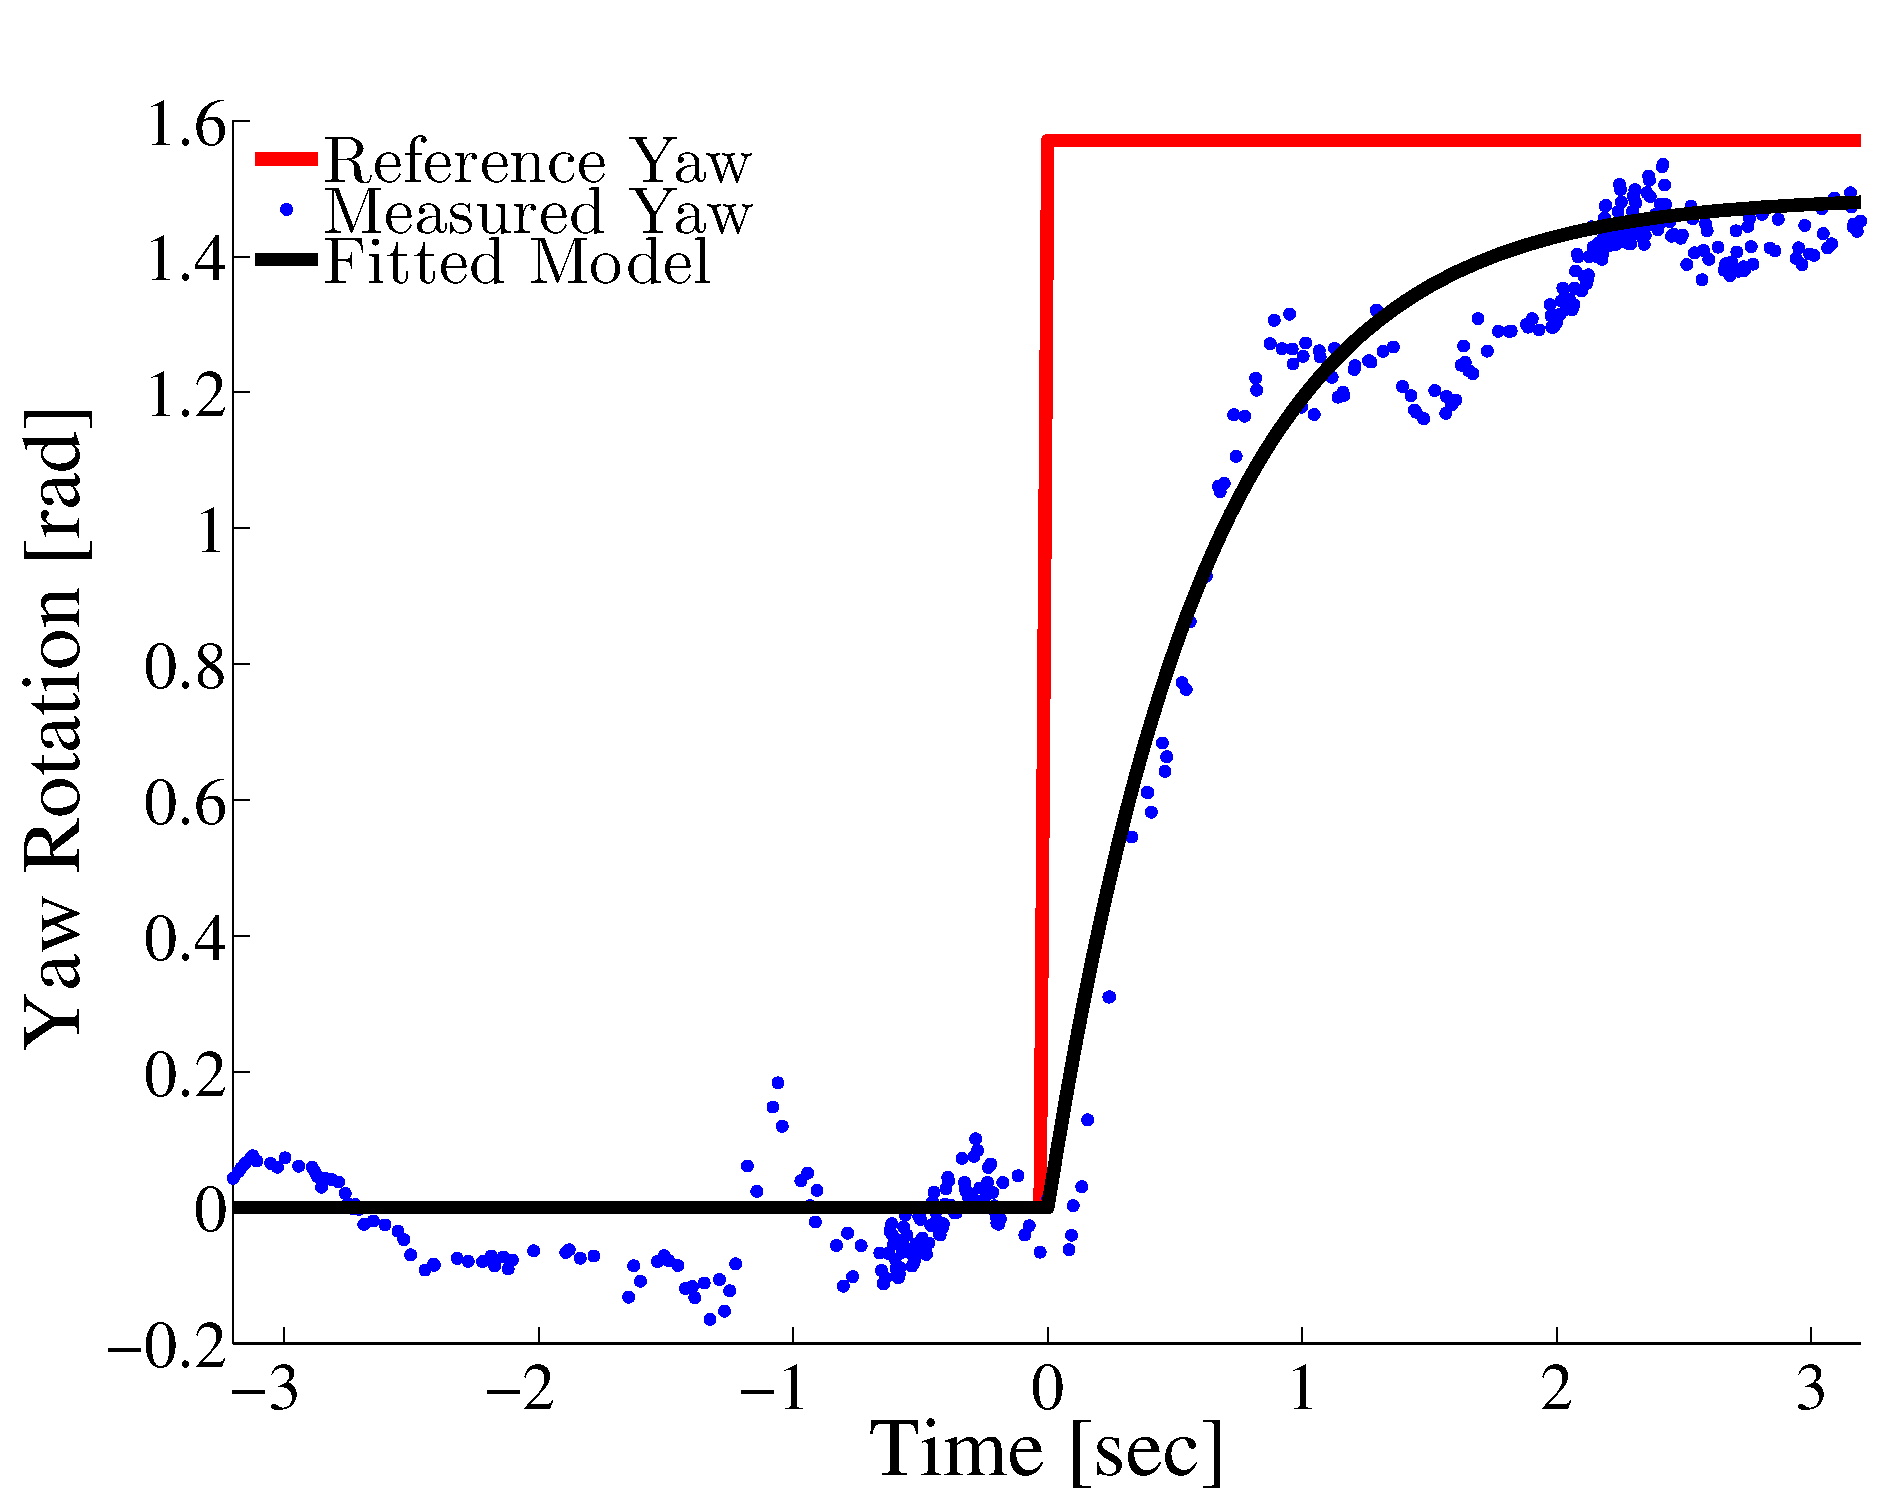
\includegraphics[width=\linewidth]{figures/step_response_total.pdf}
\caption{H$^2$Bird step response}
\label{fig:step_response}
\end{figure}

We determined the turning speed and turning radius of the H$^2$Bird
experimentally using the response of the system to the step input of a
clockwise 90 degree turn. The results of this experiment are depicted in
Figure~\ref{fig:step_response}. The data for the experiment was gathered from
the integration of the H$^2$Bird's built in gyroscope data. We used Matlab to
fit a simple low-order model, $H(s) = \frac{0.94782}{1+0.61998s}$, of the
turning behavior to the step response with the physical heading as the state
and the heading set point as the input. This model serves as a simplification
of both the turning dynamics of the ornithopter and the on-board PID
controller regulating the actuator inputs to reach the desired orientation. We
use this model in Section~\ref{sec:visual_servoing} to determine the backwards
reachable region for navigating through the window in simulation.
\\
The step response has a rise time of approximately 1.4 seconds. The H$^2$Bird
flies at an average forward velocity of 1.2 m/s, so the estimated minimum
turning radius of the robot is 1.07 meters. This flight speed is slower than
the maximum speed of the ornithopter to facilitate more reliable tracking.
%----------------------------------------------------------------------------%
\subsection{Visual Servoing}
\label{sec:visual_servoing}
%TODO cameron

%TODO make these span the page, with identical scales/style
\begin{figure*}[h]

\begin{minipage}[b]{0.45\linewidth}
\centering
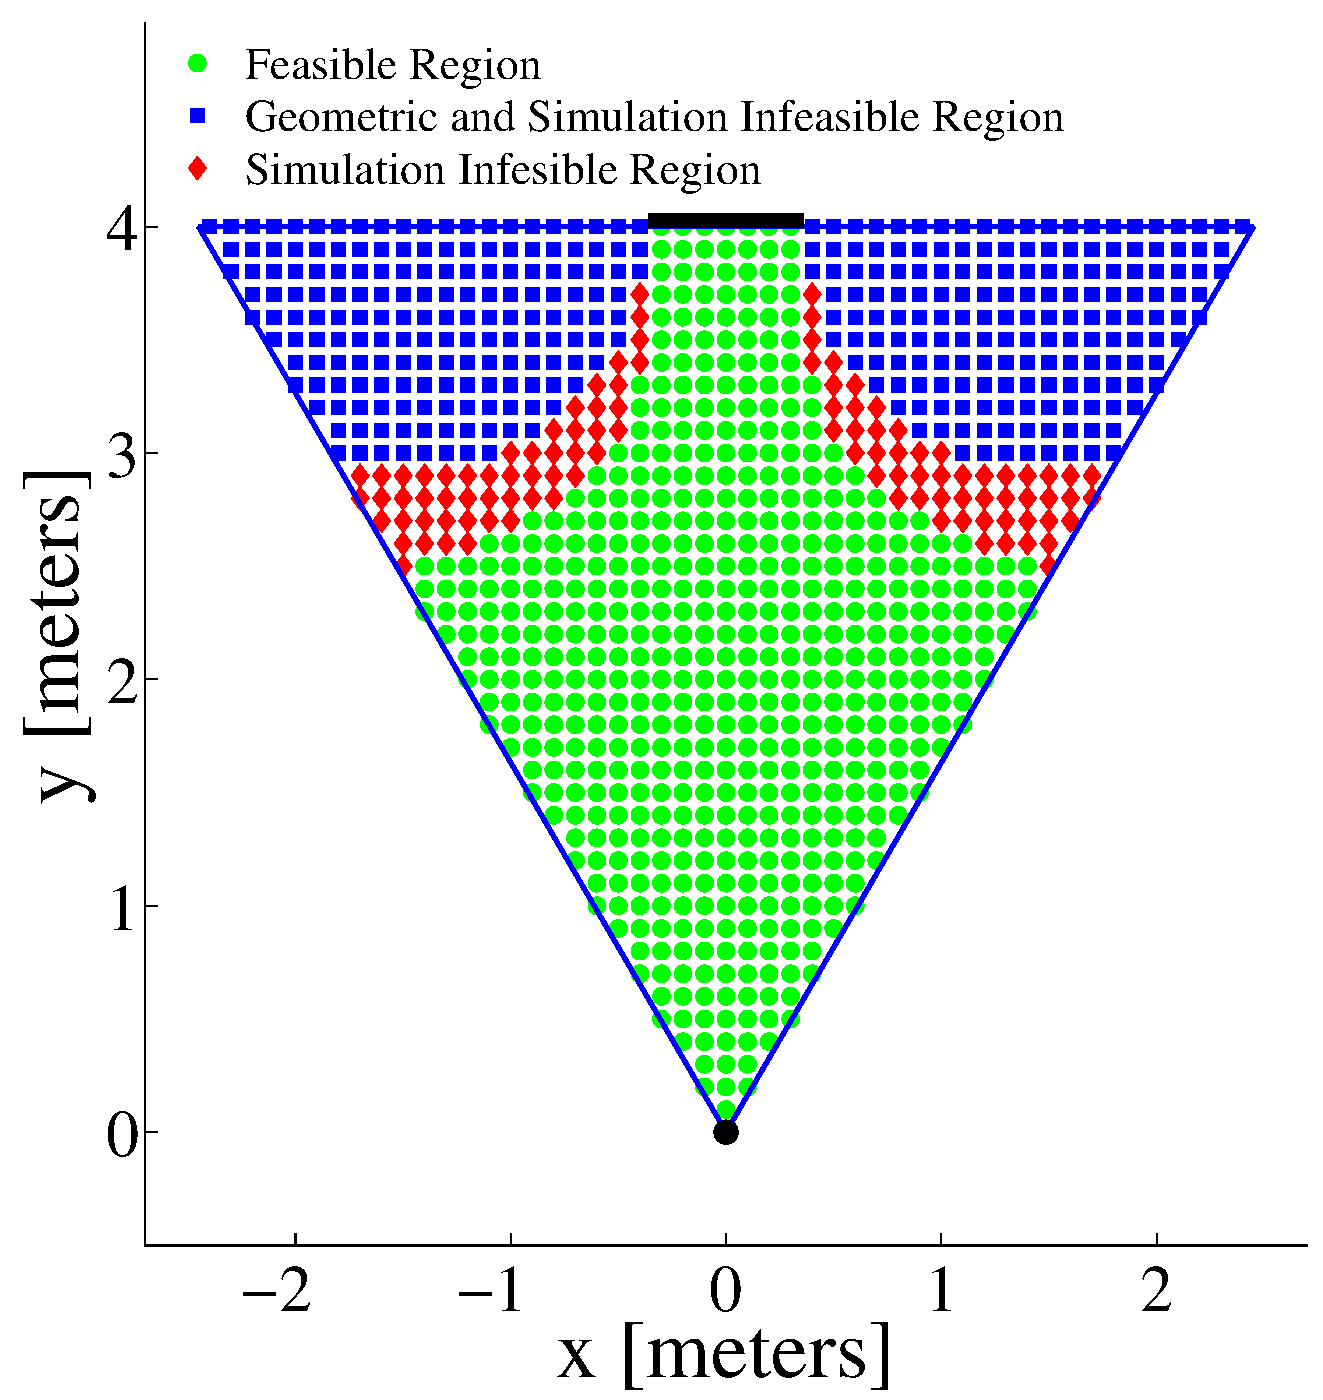
\includegraphics[width=\textwidth]{figures/feasible_set.pdf}
\caption{Plot of backwards reachable set for successful window traversal.}
\label{fig:feasible_set}
\end{minipage}

\hspace{0.5cm}
\begin{minipage}[b]{0.45\linewidth}
\centering
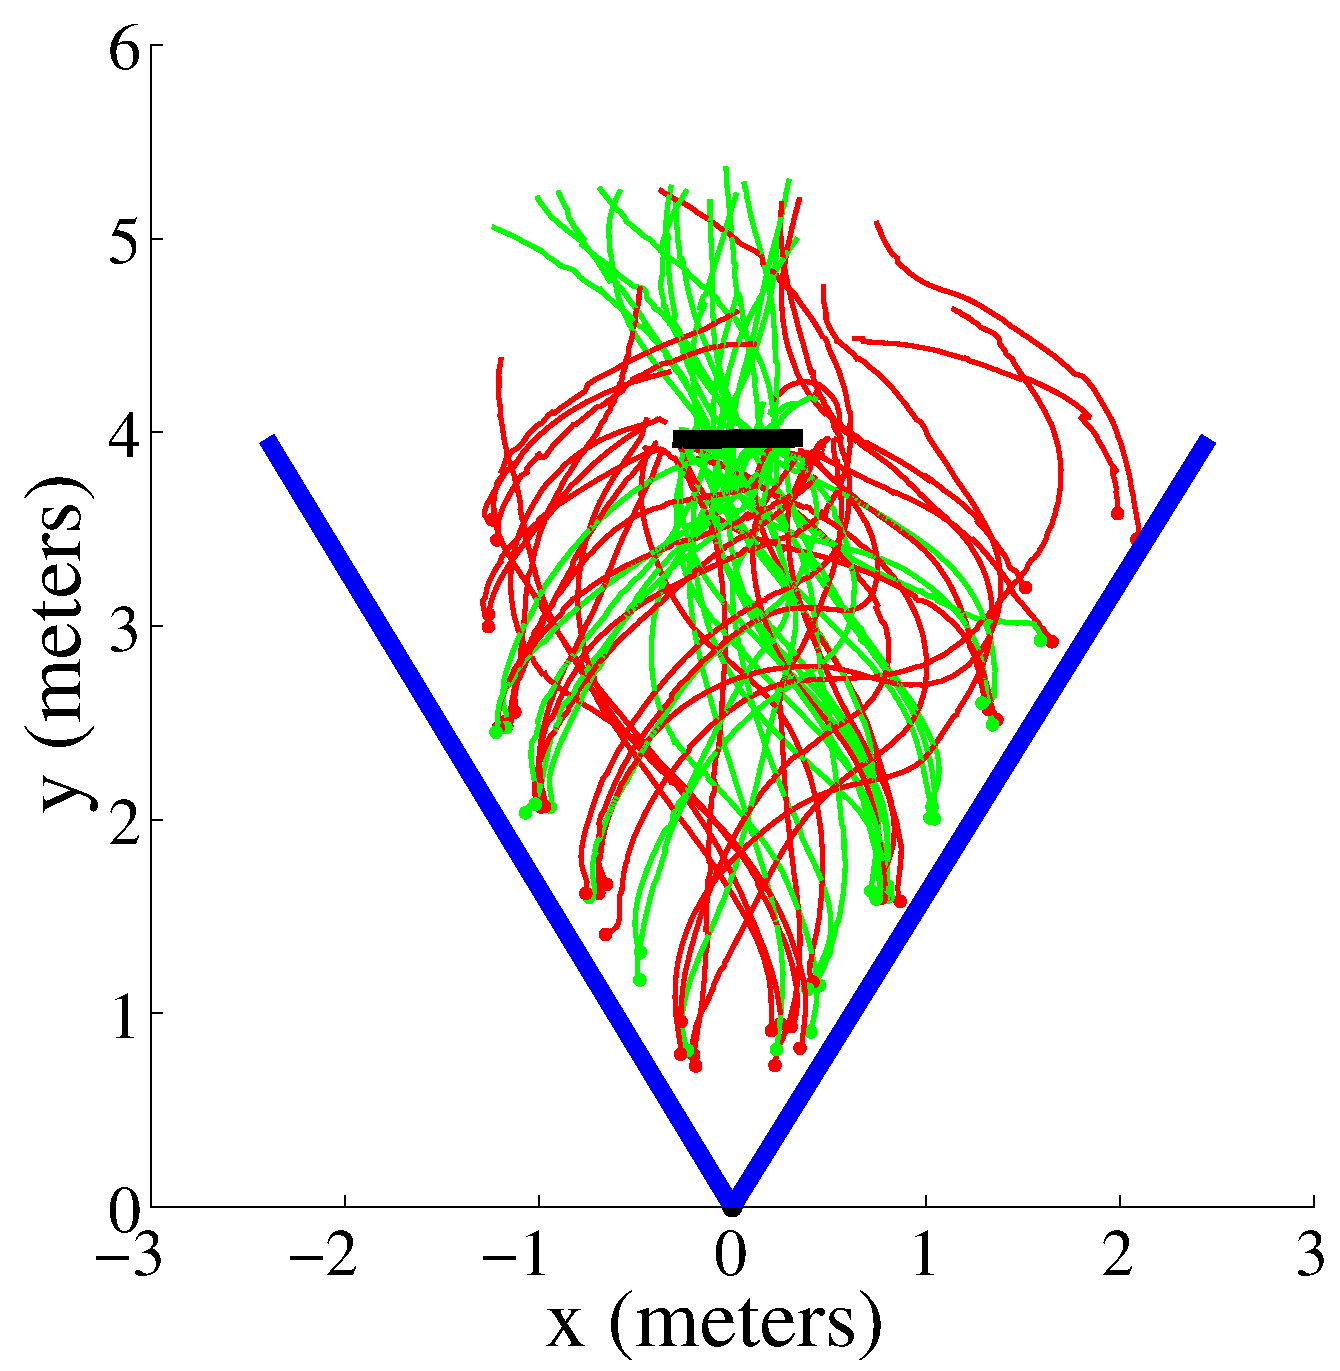
\includegraphics[width=\textwidth]{figures/flight_paths.pdf}
\caption{Plot of camera field-of-view and H$^2$Bird minimum turning radius 
cone, with experimental trials overlayed.}
\label{fig:flight_paths}
\end{minipage}

\end{figure*}

We determined the backwards reachable set of initial states for successful
window traversal both geometrically and in simulation. The results are shown
in Figure~\ref{fig:feasible_set}. The initial conditions that we chose are
spatially gridded in the camera viewing region at 0.05 meter increments and an
initial angular position perpendicular to the window plane. The geometrically
infeasible region is indicated in blue and was computed using the minimum
turning radius and simple geometry. Both the regions in red and blue indicate
the infeasible region determined in simulation. We simulated the turning model
described in Section~\ref{sec:flight_control}, with a PID controller steering
the system to the center of the window as the input. The infeasible region
calculated in simulation is a superset of the geometrically infeasible region.
The simulation is more realistic as the rotational damping during the turn and
the on-board PID controller cause the real system to react to inputs at a
non-constant angular velocity.
\\
To verify the feasible region experimentally, we conducted trials at initial
distances in X meter increments from the window along the edges of the image
frame of the camera. We started each trial with an initial heading
perpendicular to the window plane. The results of the experiments are shown in
Figure~\ref{fig:flight_paths}.
\\
%%%%%%%%%%%%%%%%%%%%%%%%%%%%%%%%%%%%%%%%%%%%%%%%%%%%%%%%%%%%%%%%%%%%%%%%%%%%%%
\section{Conclusions and Future Work}
%TODO ryan
%%%%%%%%%%%%%%%%%%%%%%%%%%%%%%%%%%%%%%%%%%%%%%%%%%%%%%%%%%%%%%%%%%%%%%%%%%%%%%
\section{Acknowledgements}
The authors would like to thank Fernando Garcia Bermudez for his 
assistance with the Vicon motion capture system, Andrew Pullin for his 
help with robot photography, and the members of the Biomimetic 
Millisystems Laboratory and the EECS community at the University of 
California, Berkeley for their advice and support.

%%%%%%%%%%%%%%%%%%%%%%%%%%%%%%%%%%%%%%%%%%%%%%%%%%%%%%%%%%%%%%%%%%%%%%%%%%%%%%%

%%%%%%%%%%%%%%%%%%%%%%%%%%%%%%%%%%%%%%%%%%%%%%%%%%%%%%%%%%%%%%%%%%%%%%%%%%%%%%%
% BIBLIOGRAPHY

% The following two commands are all you need in the
% initial runs of your .tex file to
% produce the bibliography for the citations in your paper.
\bibliographystyle{abbrv}
\bibliography{manuscript}

% ACM needs 'a single self-contained file'!
%\subsection{References}
% Generated by bibtex from your ~.bib file.  Run latex,
% then bibtex, then latex twice (to resolve references)
% to create the ~.bbl file.  Insert that ~.bbl file into
% the .tex source file and comment out
% the command \texttt{{\char'134}thebibliography}.
\end{document}
